% This is "sig-alternate.tex" V2.1 April 2013
% This file should be compiled with V2.5 of "sig-alternate.cls" May 2012
%
% This example file demonstrates the use of the 'sig-alternate.cls'
% V2.5 LaTeX2e document class file. It is for those submitting
% articles to ACM Conference Proceedings WHO DO NOT WISH TO
% STRICTLY ADHERE TO THE SIGS (PUBS-BOARD-ENDORSED) STYLE.
% The 'sig-alternate.cls' file will produce a similar-looking,
% albeit, 'tighter' paper resulting in, invariably, fewer pages.
%
% ----------------------------------------------------------------------------------------------------------------
% This .tex file (and associated .cls V2.5) produces:
%       1) The Permission Statement
%       2) The Conference (location) Info information
%       3) The Copyright Line with ACM data
%       4) NO page numbers
%
% as against the acm_proc_article-sp.cls file which
% DOES NOT produce 1) thru' 3) above.
%
% Using 'sig-alternate.cls' you have control, however, from within
% the source .tex file, over both the CopyrightYear
% (defaulted to 200X) and the ACM Copyright Data
% (defaulted to X-XXXXX-XX-X/XX/XX).
% e.g.
% \CopyrightYear{2007} will cause 2007 to appear in the copyright line.
% \crdata{0-12345-67-8/90/12} will cause 0-12345-67-8/90/12 to appear in the copyright line.
%
% ---------------------------------------------------------------------------------------------------------------
% This .tex source is an example which *does* use
% the .bib file (from which the .bbl file % is produced).
% REMEMBER HOWEVER: After having produced the .bbl file,
% and prior to final submission, you *NEED* to 'insert'
% your .bbl file into your source .tex file so as to provide
% ONE 'self-contained' source file.
%
% ================= IF YOU HAVE QUESTIONS =======================
% Questions regarding the SIGS styles, SIGS policies and
% procedures, Conferences etc. should be sent to
% Adrienne Griscti (griscti@acm.org)
%
% Technical questions _only_ to
% Gerald Murray (murray@hq.acm.org)
% ===============================================================
%
% For tracking purposes - this is V2.0 - May 2012

\documentclass{sig-alternate-05-2015}

\usepackage{hyperref}
\usepackage{verbatim}

\begin{document}

% Copyright
%\setcopyright{acmcopyright}
%\setcopyright{acmlicensed}
%\setcopyright{rightsretained}
%\setcopyright{usgov}
%\setcopyright{usgovmixed}
%\setcopyright{cagov}
%\setcopyright{cagovmixed}


% DOI
%\doi{10.475/123_4}

% ISBN
%\isbn{123-4567-24-567/08/06}

%Conference
%\conferenceinfo{PLDI '13}{June 16--19, 2013, Seattle, WA, USA}

%\acmPrice{\$15.00}


%
% --- Author Metadata here ---
%\conferenceinfo{WOODSTOCK}{'97 El Paso, Texas USA}
%\CopyrightYear{2007} % Allows default copyright year (20XX) to be over-ridden - IF NEED BE.
%\crdata{0-12345-67-8/90/01}  % Allows default copyright data (0-89791-88-6/97/05) to be over-ridden - IF NEED BE.
% --- End of Author Metadata ---

\title{Business Intelligence, 188.429 WS 2016}
\subtitle{Assignment 1}
%
% You need the command \numberofauthors to handle the 'placement
% and alignment' of the authors beneath the title.
%
% For aesthetic reasons, we recommend 'three authors at a time'
% i.e. three 'name/affiliation blocks' be placed beneath the title.
%
% NOTE: You are NOT restricted in how many 'rows' of
% "name/affiliations" may appear. We just ask that you restrict
% the number of 'columns' to three.
%
% Because of the available 'opening page real-estate'
% we ask you to refrain from putting more than six authors
% (two rows with three columns) beneath the article title.
% More than six makes the first-page appear very cluttered indeed.
%
% Use the \alignauthor commands to handle the names
% and affiliations for an 'aesthetic maximum' of six authors.
% Add names, affiliations, addresses for
% the seventh etc. author(s) as the argument for the
% \additionalauthors command.
% These 'additional authors' will be output/set for you
% without further effort on your part as the last section in
% the body of your article BEFORE References or any Appendices.

\numberofauthors{2} %  in this sample file, there are a *total*
% of EIGHT authors. SIX appear on the 'first-page' (for formatting
% reasons) and the remaining two appear in the \additionalauthors section.
%
\author{
% You can go ahead and credit any number of authors here,
% e.g. one 'row of three' or two rows (consisting of one row of three
% and a second row of one, two or three).
%
% The command \alignauthor (no curly braces needed) should
% precede each author name, affiliation/snail-mail address and
% e-mail address. Additionally, tag each line of
% affiliation/address with \affaddr, and tag the
% e-mail address with \email.
%
% 1st. author
\alignauthor
Stefan Beyer\\
       \affaddr{Student ID: 1225423}\\
       \email{e1225423@student.tuwien.ac.at}
% 2nd. author
\alignauthor
Georg Heiler\\
       \affaddr{Student ID: 1225063}\\
       \email{e1225063@student.tuwien.ac.at}
}
% There's nothing stopping you putting the seventh, eighth, etc.
% author on the opening page (as the 'third row') but we ask,
% for aesthetic reasons that you place these 'additional authors'
% in the \additional authors block, viz.
\date{30 July 1999}
% Just remember to make sure that the TOTAL number of authors
% is the number that will appear on the first page PLUS the
% number that will appear in the \additionalauthors section.

\maketitle

\section{Dataset}
We use the \href{https://www.kaggle.com/c/leaf-classification}{leaf classification dataset from Kaggle}. The idea is to automate plant recognition. The data consists of binary leaf images and extracted features, including shape, margin \& texture, to accurately identify 99 species of plants.

\subsection{Characteristics of the extracted features}
The following numbers are for the training data set

\begin{itemize}
  \item Number of features 194
  \item Number of categorical features 1
  \item Number of numerical features 193
  \item Number of Samples 990
  \item Target variable contains 99 different species
\end{itemize}

The test data set contains 594 additional instances. All in all the minimum requirements for the dataset are fulfilled.


A detailed description of mean / min values or value ranges can be found in 
\textbf{firstAnalysisOfTheData}
, including histograms. 

In general:
\begin{itemize}
  \item id
  \item ID of the images from which the features were extracted
  \item Range: [1,1584]
  \item marginN (1-64)
  \begin{itemize}
	  \item Numerical
	  \item Range (approximately): [0,0.3]
	  \item Many outliers
  \end{itemize}
  \item shapeN (1-64)
  \begin{itemize}
 	  \item Numerical
	  \item Range (approximately): [0,0.003]
	  \item Few outliers
\end{itemize}
\item textureN (1-64)
	\begin{itemize}
		\item Numerical
	  \item Range (approximately): [0,0.43]
	  \item Few outliers
\end{itemize}

\item species
  \begin{itemize}
	\item Categorical
	  \item 99 unique values
	  \item The dataset does not contain any missing values and is not sparse.
\end{itemize}

\end{itemize}

\section{Classification}
Analysis of Train/Test Set Splits, Performance and Parameters

\subsection{Selection of algorithms}
\subsubsection{Logistic regression (extracted features)}
\begin{itemize}
  \item results easy to interpret
  \item fast to compute
\end{itemize}

Parameters:
\begin{itemize}
  \item C: inverse of the regularization strength
  \item solver: algorithm to use in the optimization problem
\end{itemize}


\subsubsection{Random forest (extracted features)}
\begin{itemize}
  \item popular methodology
  \item no feature scaling required
  \item very robust
  \item quick for smaller datasets
\end{itemize}

Parameters:
\begin{itemize}
  \item n\_estimators: number of trees
  \item criterion: criterion used for splits of the trees
  \item min\_samples\_leaves: minimum number of samples required to be a leaf node 
\end{itemize}

\subsection{Preprocessing}

\subsubsection{Scaling}
marginN, scaleN and textureN will be scaled, we will explore the results of different scaling algorithms later on (standardization and min-max scaling) via pipelines to streamline the workflow.
An example for the min-max scaler is displayed below:
\begin{verbatim}
Pipeline([('scaling', MinMaxScaler()),
          ('estimator', LogisticRegression(...))])
\end{verbatim}

\subsubsection{Target variable}

Label encoding of target variable:
\begin{verbatim}
df.species = df.species.astype('category').cat.codes
\end{verbatim}

Splitting data frame into training data X and labels y and ID column:
\begin{verbatim}
def transform(data):
    ID = data.id
    X = data.drop(['species', 'id'], axis=1)
    y = data['species']
    return ID, X, y

ID, X, y = transform(df)
\end{verbatim}

The ID column is a reference to the original image and not suited for training, as it conveys no meaning.

\subsubsection{Additional preprocessing}
For marginN and textureN we will introduce a new column with binary values which will be 1 if the value of marginN / textureN is nearly 0.
We do this in order to better handle numeric distances which otherwise might get distorted.

\begin{verbatim}
def addZeroColumn(df, colName):
    df.loc[df[colName] < 0.01, 
          colName + '_is_small'] = 1
    df[colName + '_is_small']
         .fillna(0, inplace=True)

def addZeroColumns(df, colBaseName):
    for n in range(1,65):
        addZeroColumn(df, colBaseName + str(n))
        
addZeroColumns(X, 'margin')
addZeroColumns(X, 'texture')
\end{verbatim}

\subsection{Subsampling}
We will process the entire dataset, as it only contains around 1000 rows.

\section{Training \& Testing}
The code to follow along with this part of the assignment can be found in \emph{02\_classification.ipnb}. Below only the obtained results will be discussed.
\subsection{Quality metrics}

We chose the following quality metrics:
\begin{itemize}
	\item Precision Score
	\item Recall Score
	\item Accuracy Score
	\item Cohen Kappa Score
	\item F1 Score
\end{itemize}

To calculate those metrics we calculated the mean over the 10 folds.
For some metrics (precision, recall, f1) we averaged the results over all classes beforehand, because all classes are equally distributed, stratified sampled in cross-validation and all classes are equally important.

\subsection{Parameters}

\subsubsection{Logistic Regression}
The combinations of parameters can be seen in the table below.

\begin{table}[h]
\label{tbl:1}
\centering
\caption{Parameters for logistic regression}
\begin{tabular}{|c|c|}
\hline 
Solver & C \\ 
\hline 
lbfgs & 1 \\ 
\hline 
lbfgs & 0.8 \\ 
\hline 
lbfgs & 1.2 \\ 
\hline 
lbgfs & 10 \\ 
\hline 
newton-cg & 1 \\ 
\hline 
newton-cg & 0.8 \\ 
\hline 
newton-cg & 1.2 \\ 
\hline 
newton-cg & 10 \\ 
\hline 
\end{tabular} 
\end{table}

We experienced similar results with all parameter combinations.
In Figure \ref{fig:lr} the results for the first set of parameters is shown.

\begin{figure}[h]
  \label{fig:lr}
  \centering
  \caption{Logistic regression with solver=lbfgs, C=1}
  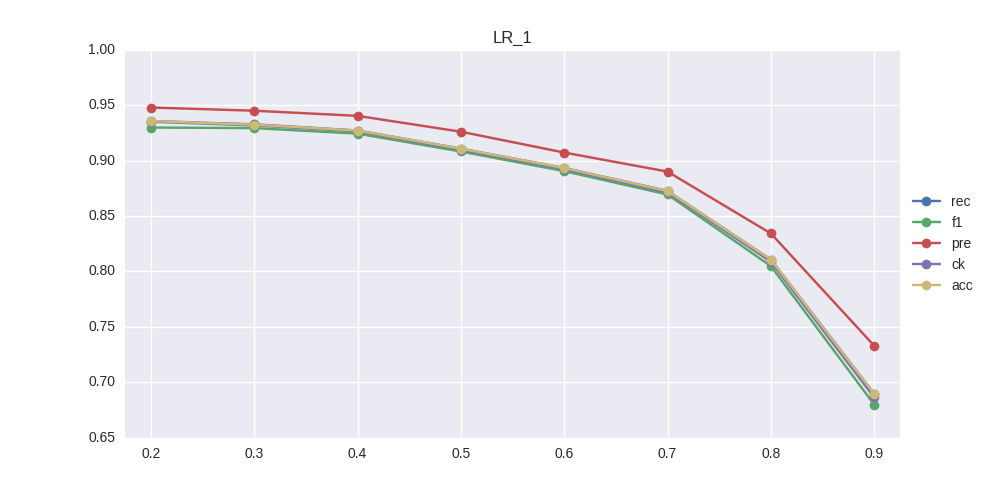
\includegraphics[width=0.5\textwidth]{../plots/LR_1}
  \label{fig:anomalySetup}
\end{figure}

\subsubsection{Random Forest}


\subsection{Scaling}

\subsection{Training / test set split}


\end{document}
